\subsubsection{Exception}

\label{Exception}
\begin{figure}[ht]
	\centering
	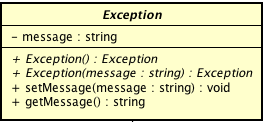
\includegraphics[scale=0.5]{Sezioni/SottosezioniST/img/app/Exception.png}
	\caption{Exception}
\end{figure}

\begin{itemize}
\item \textbf{Descrizione}: Classe base astratta per le eccezioni lanciate dai metodi della libreria Monolith.
\item \textbf{Utilizzo}: Lo sviluppatore può estendere questa classe per creare delle classi di eccezioni personalizzate più specifiche di sua utilità.
\item \textbf{Attributi}: 
	\begin{itemize}
	\item \textit{private message:string}\\
	Il messaggio d'errore testuale lanciato dall'eccezione.
	\end{itemize}
\item \textbf{Metodi}:
	\begin{itemize}
	\item \textit{public Exception():Exception}\\
	Il costruttore senza parametri della classe Exception.
	\item \textit{public Exception(message:string):Exception}\\
	Il costruttore con un parametro per il messaggio d'errore della classe Exception.
			\item{\textbf{Parametri}: \begin{itemize}
			\item \textit{message:string}\\
			Il messaggio d'errore che si vuole impostare per l'eccezione.
			\end{itemize}}
	\item \textit{public setMessage(message:string):void}\\
	Imposta un messaggio d'errore per l'eccezione.
			\item{\textbf{Parametri}: \begin{itemize}
			\item \textit{message:string}\\
			Il messaggio d'errore che si vuole impostare per l'eccezione.
			\end{itemize}}
	\item \textit{public getMessage():string}\\
	Ritorna una stringa contenente il messaggio d'errore dell'eccezione.
	\end{itemize}
\item \textbf{Eventi}:
\end{itemize}

\subsubsection{BadParameterException}

\label{BadParameterException}
\begin{figure}[ht]
	\centering
	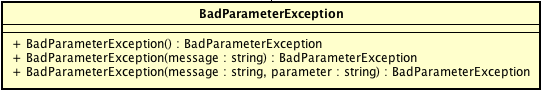
\includegraphics[scale=0.5]{Sezioni/SottosezioniST/img/app/BadParameterException.png}
	\caption{BadParameterException}
\end{figure}

\begin{itemize}
\item \textbf{Descrizione}: Classe di eccezione che deriva da Exception.
\item \textbf{Utilizzo}: Le eccezioni che appartengono a questa classe vengono lanciate nel caso in cui un parametro di un metodo chiamato è scorretto.
\item \textbf{Attributi}: 
\item \textbf{Metodi}:
	\begin{itemize}
	\item \textit{public BadParameterException():BadParameterException}\\
	Il costruttore senza parametri della classe BadParameterException.
	\item \textit{public BadParameterException(message:string):BadParameterException}\\
	Il costruttore con un parametro per il messaggio d'errore della classe BadParameterException.
			\item{\textbf{Parametri}: \begin{itemize}
			\item \textit{message:string}\\
			Il messaggio d'errore che si vuole impostare per l'eccezione.
			\end{itemize}}
	\item \textit{public BadParameterException(message:string,parameter:string):BadParameterException}\\
	Il costruttore con due parametri per il messaggio d'errore e il parametro che ha causato l'errore della classe BadParameterException.
			\item{\textbf{Parametri}: \begin{itemize}
			\item \textit{message:string}\\
			Il messaggio d'errore che si vuole impostare per l'eccezione.
			\item \textit{message:string}\\
			La stringa contenente il parametro che ha causato l'eccezione.
			\end{itemize}}
	\end{itemize}
\item \textbf{Eventi}:
\end{itemize}